\title{Practice with Latitude and Longitude}
\author{Dr. Jordan Hanson - Whittier College Dept. of Physics and Astronomy}
\date{\today}
\documentclass[12pt]{article}
\usepackage[margin=1.25cm]{geometry}
\usepackage{hyperref}
\usepackage{graphicx}
\usepackage{amsmath}
\begin{document}
\twocolumn
\maketitle
\small

\section{Introduction}

\textit{Latitude} and \textit{longitude} are two angles that we use to locate objects on the surface of the Earth.  The latitude angle $\theta$ relates the radius of the Earth, $R$, to a distance traveled in the North-South direction, $s$.  These three variables are related as follows:

\begin{equation}
s = R\theta \label{eq:lat}
\end{equation}

The longitude angle $\phi$ relates the radius of the Earth, $R$, to a distance traveled in the East-West direction, $s$, and the latitude $\theta$.  These four variables are related as follows:

\begin{equation}
s = \phi R \cos\theta \label{eq:lon}
\end{equation}

The term $\cos\theta$ means ``the cosine of theta.''  The cosine of an angle within a right triangle is equal to the adjacent leg of the right triangle, divided by the hypotenuse.  The angles $\theta$ and $\phi$ are given in \textit{radians}, or unitless numbers that correspond to raw angle.  For example, since the circumference of a circle is $C = 2\pi r$, where $r$ is the radius, then 360 degrees is equal to $2\pi$ radians (see Eq. \ref{eq:lat}).

In Sec. \ref{sec:deg}, we learn how to interpret latitude and longitude using the system of degrees, minutes, and seconds.  In Sec. \ref{sec:exer}, we will practice computing the latitude and longitude, given our distances traveled.  In Sec. \ref{sec:whit}, we will locate the coordinates of Whittier College, and learn how to write them in degree-minute-second form.
 
\begin{figure}
\centering
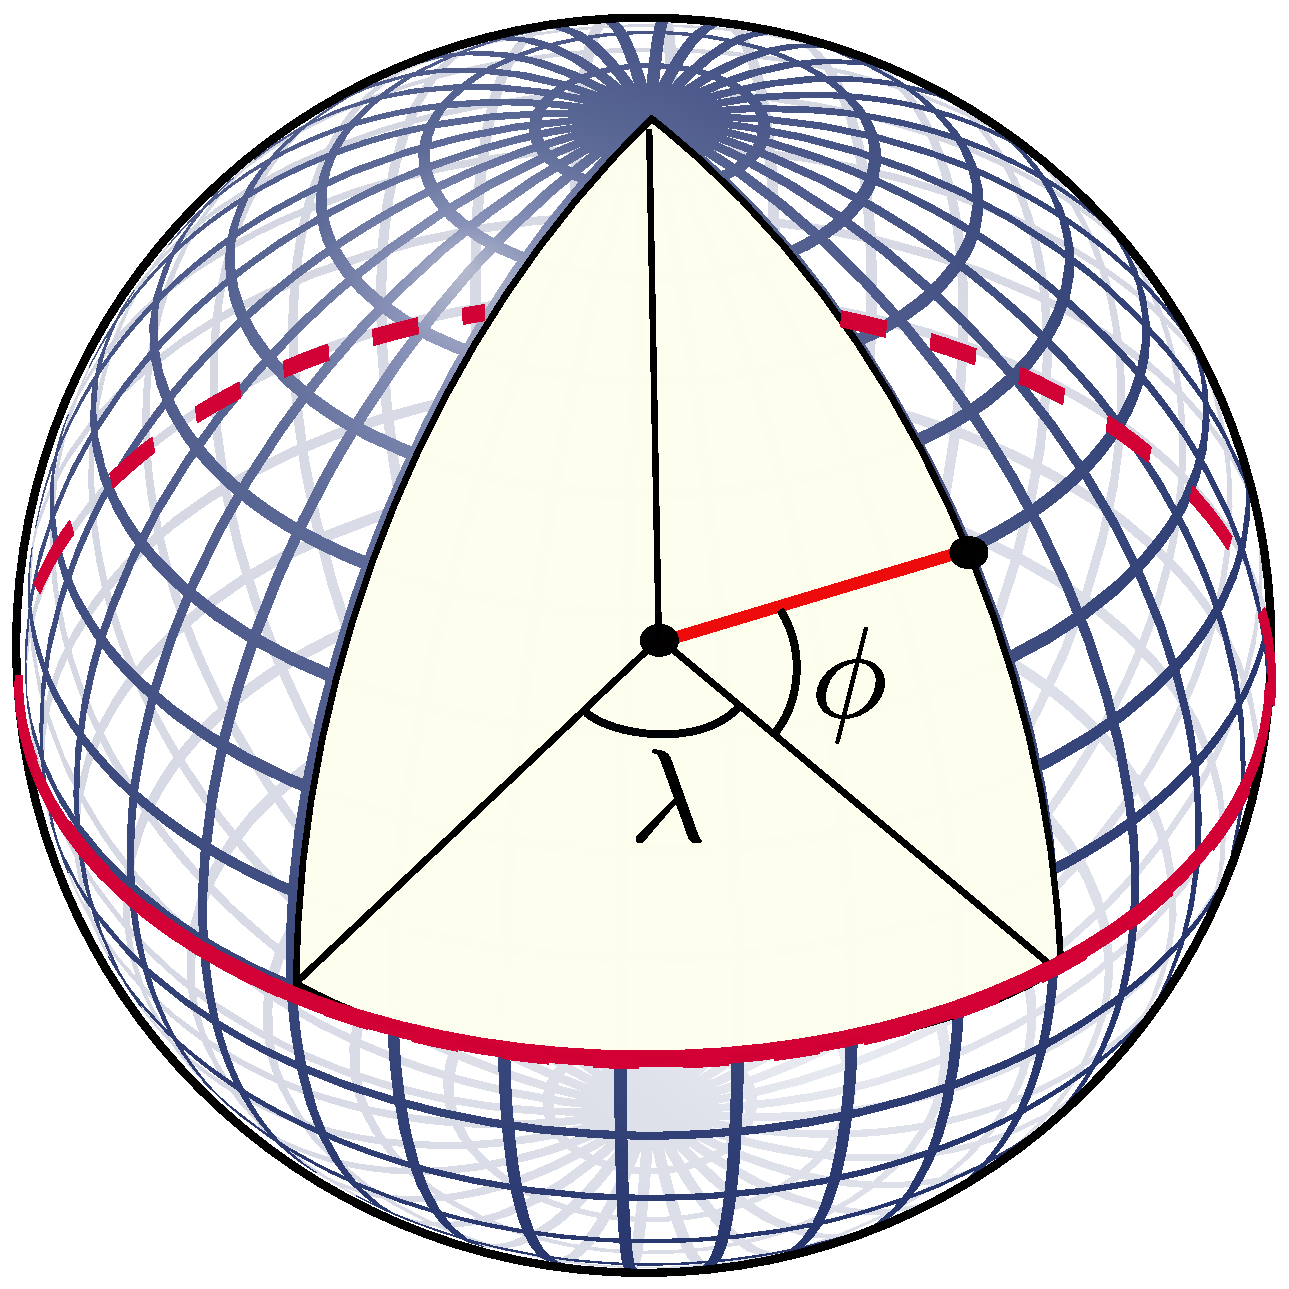
\includegraphics[width=0.25\textwidth]{latlon.pdf}
\caption{\label{fig:latlon} A position on a sphere can be described by two locations or angles.}
\end{figure}

\section{Converting to Degrees}
\label{sec:deg}

The value $2\pi$ radians is equal to 360 degrees, so the conversion factor is $180/\pi$ (degrees per radian).  To convert radians to degrees, multiply by $180/\pi$.  To undo this conversion, multiply by $\pi/180$.

\begin{enumerate}
\item Convert $\pi/4$ radians to degrees.
\item Convert $3\pi/2$ radians to degrees.
\item Convert 90 degrees to radians.
\item Convert 60 degrees to radians.
\end{enumerate}

Suppose you find an angle in radians with a decimal number, like 60.5 degrees.  The usual way we express latitude and longitude does not involve decimals.  Instead, we use \textit{minutes} and \textit{seconds}.  There are 60 minutes in 1 degree, and there are 60 seconds in 1 minute of one degree.  Thus, 60.5 degrees would be written as ``60 degrees, and 30 minutes,'' or $60^{\circ}, 30'$.  We also have to specify North or South of the equator for latitude, and East or West of the \textit{meridian} for longitude.  Use Google maps to determine the location of the meridian in the current system of longitude.

\section{Calculating the Latitude and Longitude}
\label{sec:exer}

Complete the following exercises using Eq. \ref{eq:lat}.

\begin{enumerate}
\item Suppose a traveler sails down a river that runs directly North and South.  If he travels for 200 km, and the radius of the Earth is 6,371 km, what is the change in latitude? \\ \vspace{2cm}
\item If he travels North, and his instruments tell him he moved 2 degrees North, how far in kilometers did he move? \\ \vspace{2cm}
\end{enumerate}

Complete the following exercises using Eq. \ref{eq:lon}.

\begin{enumerate}
\item Suppose a traveler sails down a river that runs directly East and West.  Her current latitude is $+\pi/4$ (45 degrees North of the equator).  If she travels West for 200 km, and the radius of the Earth is 6,371 km, what is the change in longitude? \\ \vspace{2cm}
\item If she travels East (same latitude), and her instruments tell her she moved 1/80 degrees East, how far in kilometers did she move? \\ \vspace{2cm}
\end{enumerate}

\section{Locate Whittier College}
\label{sec:whit}

\begin{enumerate}
\item Using Google Maps, (a) locate Whittier College and give the proper coordinates, in latitude and longitude, of the Science and Learning Center. (b) The coordinates are likely in decimal form. Using the fact that one \textit{minute} equals 1/60th of a degree, and one \textit{second} equals 1/60th of a minute, convert our coordinates to degree-minute-second form.
\item \textbf{Bonus:} (a) Compute the number of kilometers per degree change in latitude, along a fixed longitude. (b) Compute the number of kilometers per minute change in latitude, along a fixed longitude.
\item Note: a latitude of zero means we are at the North Pole.  A longitude of zero means we are along the meridian.
\end{enumerate}

\end{document}
